\documentclass[a4paper,UTF8]{article}
\usepackage{ctex}
\usepackage[margin=1.25in]{geometry}
\usepackage{color}
\usepackage{graphicx}
\usepackage{amssymb}
\usepackage{amsmath}
\usepackage{amsthm}
\usepackage{bm}
\usepackage{hyperref}
\usepackage{float}
\numberwithin{equation}{section}
%\usepackage[thmmarks, amsmath, thref]{ntheorem}
\theoremstyle{definition}
\newtheorem*{solution}{Solution}
\newtheorem*{prove}{Proof}
\usepackage{multirow}

%--

%--
\begin{document}
\title{机器学习导论\\
习题三}
\author{151250104, 卢以宁, kiwiloveskiwis@gmail.com}
\maketitle
\section{[30pts] Decision Tree Analysis}
决策树是一类常见的机器学习方法,但是在训练过程中会遇到一些问题。

(1) \textbf{[15pts]} 试证明对于不含冲突数据(即特征向量完全相同但标记不同)的训练集,必存在与训练集一致(即训练误差为0)的决策树; 

(2) \textbf{[15pts]} 试分析使用“最小训练误差”作为决策树划分选择的缺陷。
\begin{solution} \,

(1)反设不存在训练误差为0的决策树,则必存在训练误差最小的决策树,设其值为$\lambda > 0$. 则必存在测试样例$D_i$被划分错误。此时,设$D_i$所属叶子节点为$Node_i$, 有如下两种情况:

1. $Node_i$仅包含$D_i$一个样例,此时将$Node_i$的类别标记改为$D_i$的类, 训练误差减小. 

2. $Node_i$ 包含多于$D_i$的数个样例。由于各节点的特征向量各不相同, 我们可重复构造以$Node_i$为根节点的子树, 重复划分直到存在某叶节点只包含$D_i$一个样例,  将其类别标记改为$D_i$所属类,  其余叶节点的标记维持不变。训练误差减小。

故与上述假设矛盾。故存在训练误差为0的决策树。

(2) 缺乏泛化性能,容易过拟合。例如, 在连续属性学习中,各个训练样例特征向量完全相同的概率很小, 此时我们可以按照(1)题的方式构造训练误差接近于0的决策树。但这样的坏处是过于针对训练数据,从而可能泛化误差更大。

\end{solution}

\section{[30pts] Training a Decision Tree}
考虑下面的训练集:共计6个训练样本,每个训练样本有三个维度的特征属性和标记信息。详细信息如表\ref{table:training}所示。

请通过训练集中的数据训练一棵决策树,要求通过“信息增益”(information gain)为准则来选择划分属性。请参考书中图4.4,给出详细的计算过程并画出最终的决策树。
\begin{table}[H]
\centering
\caption{训练集信息}
\label{table:training}\vspace{2mm} 
\begin{tabular}{c|c c c|c}\hline
序号		&  特征 \textbf{A} 	&	特征 \textbf{B}	&	特征 \textbf{C} 	&	标记    \\ \hline
1		&  0 	&	1	&	1 	&	0    \\
2		&  1 	&	1 	&	1 	&	0    \\
3		&  0 	&	0 	&	0 	&	0    \\
4		&  1 	&	1 	&	0 	&	1    \\
5		&  0 	&	1 	&	0 	&	1    \\
6		&  1 	&	0 	&	1 	&	1    \\\hline
\end{tabular} 
\end{table}

\begin{solution}
\begin{equation}
\begin{split}
Ent(D) &= - \sum_{k=1}^2p_k\log_2p_k = - (\frac{1}{2}\log_2\frac{1}{2} \cdot 2 ) = 1 \\ 
Gain (D, feature) &= Ent(D) - \sum_{v=1}^2 \frac{|D^v|}{|D|} Ent(D^v) \\
Gain (D, A) &= 1 - (\frac{1}{2} \cdot  0.918 \cdot 2) = 0.082 \\
Gain (D, B) &= 1- (\frac{1}{2} \cdot 1 \cdot 2)  = 0 \\
Gain (D, C) &= 1 - (\frac{1}{2} \cdot  0.918 \cdot 2)  = 0.082 
\end{split}
\end{equation}
由于$Gain (D, A) = Gain (D, C)$ , 任选其一作为划分属性。尝试选择属性A。将$A=0$的训练样本划分为$D^1$, $A=1$的为 $D^2$ , 则 \\
\begin{equation}
\begin{split}
Ent(D^1) &= 0.918, Ent(D^2) = 0.928 \\
Gain (D^1, B) &=   0.918 - (\frac{1}{3} \cdot 0 +  \frac{2}{3} \cdot 1)  = 0.251 \\
Gain (D^1, C) &= Gain (D^2, B) =  Gain (D^2, C)  = 0.251
\end{split}
\end{equation}
在根节点为属性A的情况下, 我们必须进一步划分节点才能够达到\%100的纯度. 但是, 若我们选择属性C作为划分节点, 将$C=0$的训练样本划分为$D^1$, $C=1$的为 $D^2$ , 则 \\
\begin{equation}
\begin{split}
Ent(D^1) &= 0.918, Ent(D^2) = 0.928 \\
Gain (D^1, A) &= Gain (D^2, A)   = 0.918 - (\frac{1}{3} \cdot 0 +  \frac{2}{3} \cdot 1)  = 0.251 \\
Gain (D^1, B) &=  Gain(D^2, B) = 0.928
\end{split}
\end{equation}
可在只划分两次的基础上达到百分百的准确率。 故选取A为根节点划分属性, B为$D^1$、$D^2$的划分属性, 最终决策树如下。
\begin{figure}[H]{}
\centering 
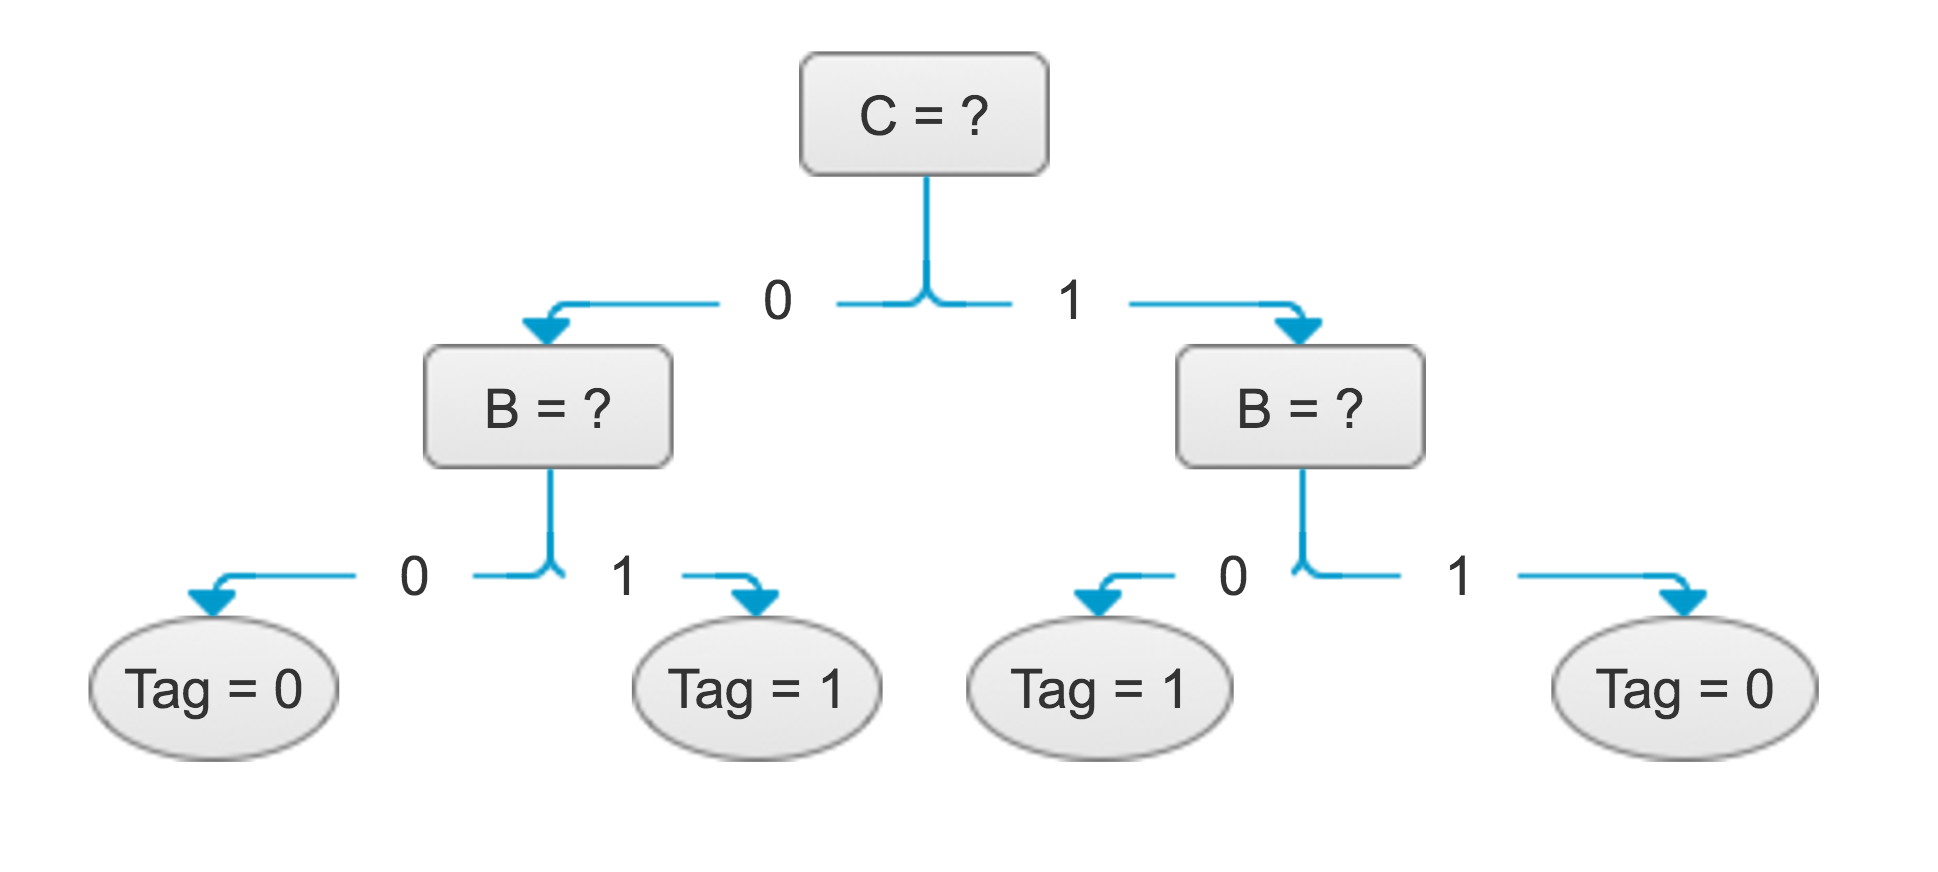
\includegraphics[scale=0.3]{tree.png}
\caption{Decision Tree of Table 1 }
\end{figure} 
\end{solution}


\section{[40pts] Back Propagation} 
单隐层前馈神经网络的误差逆传播(error BackPropagation,简称BP)算法是实际工程实践中非常重要的基础,也是理解神经网络的关键。

请编程实现BP算法,算法流程如课本图5.8所示。详细编程题指南请参见链接:\url{http://lamda.nju.edu.cn/ml2017/PS3/ML3_programming.html}

在实现之后,你对BP算法有什么新的认识吗?请简要谈谈。
\begin{solution}

Sigmoid 的导数性质省去了很多计算, 且具有对阶跃函数良好的拟合, 计算BP的时候相对方便。 \\ 
learn\_rate 分别尝试设为0.1, 0.5 和 0.8, epoch 分别尝试设为100, 150, 200, 500, 最终在考虑时间消耗的情况下选取learn\_rate为0.5, epoch为200. 最终测试集上精度约为93.7\% \\
略微困惑的是, 将数据归一化步骤略去后,测试集上的准确度提高了1.*个百分点。

\end{solution}

\section*{附加题   [30pts] Neural Network in Practice}
在实际工程实现中,通常我们会使用已有的开源库,这样会减少搭建原有模块的时间。因此,请使用现有神经网络库,编程实现更复杂的神经网络。详细编程题指南请参见链接:\url{http://lamda.nju.edu.cn/ml2017/PS3/ML3_programming.html}

和上一题相比,模型性能有变化吗?如果有,你认为可能是什么原因。同时,在实践过程中你遇到了什么问题,是如何解决的?
\begin{solution}

性能没有发生太大改变。

\end{solution}

\end{document}